\documentclass[11pt]{article}
\usepackage[utf8]{inputenc}
\usepackage[T1]{fontenc}
\usepackage{amsmath}
\usepackage{amsfonts}
\usepackage{amssymb}
\usepackage[version=4]{mhchem}
\usepackage{stmaryrd}
\usepackage{graphicx}
\usepackage[export]{adjustbox}
\graphicspath{ {./images/} }

\begin{document}
\section*{Reading}
Binomial Tree Models

Binomial trees can be used to model a variety of risks, from equities to interest rates. Binomial models are often used as no-arbitrage models to value risky securities, especially financial derivatives. This section discusses an important arbitrage-free model for a call option using a binomial tree. A call option is a financial derivative that provides its owner with the right (but not the obligation) to purchase an asset at a prespecified price on (or perhaps before) the option's expiration date. Options are discussed in detail in the Derivatives and Risk-Neutral Valuation session.

\section*{The Mechanics of a Binomial Tree That Lead to a Normal Distribution}
A binomial tree projects possible outcomes in a variable such as a security price or interest rate by modeling uncertainty as two movements: an upward movement and a downward movement. The movements are often modeled so that a pathway with an upward movement followed by a downward movement "recombines" with a pathway with a downward movement followed by an upward movement. The next exhibit illustrates how the current stock price in a binomial tree $(S)$ can move up to $S_{u}$ or down to $S_{d}$ in the first step, moving from left to right. The second time step depicts the stock price as being one of three possible values under the very helpful (but not always necessary) recombining assumption that the stock price experiencing a downward move after an upward move ( $\left.S_{u d}\right)$ is the same as one experiencing an upward move after a downward move $\left(S_{d u}\right)$. Trees recombine when upward movements are formed via a multiplicative shift factor, $S_{u}=S \times(1+u)$ , and downward movements are formed via division by the same factor, $S_{d}=S /(1+u)$. A recombining binomial tree has $n+1$ possible final outcomes for an $n$ period tree, rather than $2^{n}$ outcomes, and is therefore much more manageable for models with 30 or more time steps, since $2^{30}$ exceeds 1 billion, while a recombining 30 -step tree would have 31 final outcomes.

\begin{center}
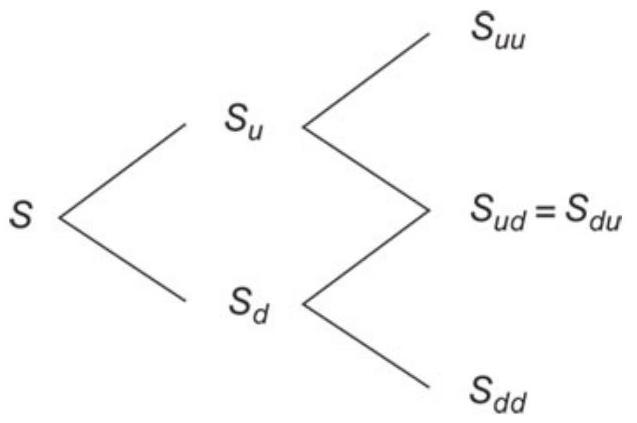
\includegraphics[max width=\textwidth]{2024_04_10_859893730bbb41b27826g-2}
\end{center}

\section*{A Two-Step Binomial Tree for a Stock Price $(S$ )}
Each step occurs over a unit of time specified by the modeler. An analyst may model a one-month period using 30 daily steps or a one-year period using 52 weekly steps. A key attribute of most binomial trees is that as the number of steps used increases (i.e., as the total time period is broken into smaller and smaller steps), the terminal distribution of the asset approaches a normal distribution. Therefore, the values obtained from the binomial model approach the values obtained using mathematical models (discussed in the session entitled Derivatives and Risk-Neutral Valuation) that assume normally distributed returns.

\section*{A Simplified Binomial Tree Model for a Stock and a Call Option}
As an illustration of the simplicity and power of these models, consider a very simplified scenario in which a stock price currently at $\$ 7$ per share is expected to rise over the next year to $\$ 12$ per share or fall to $\$ 0$ per share, depending on the outcome of a very important event. Further, assume that there is a call option on that stock with a strike price (or exercise price) of $\$ 9$ per share that expires in one year. At expiration, the call option will pay $\$ 3$ if the stock rises to $\$ 12$ (its excess above its strike price), or $\$ 0$ if the stock falls to $\$ 0$. The exhibit, Binomial Trees for Stock and Call Option with $\$ 9$ Strike, illustrates single-period binomial trees for the stock and the call option.\\
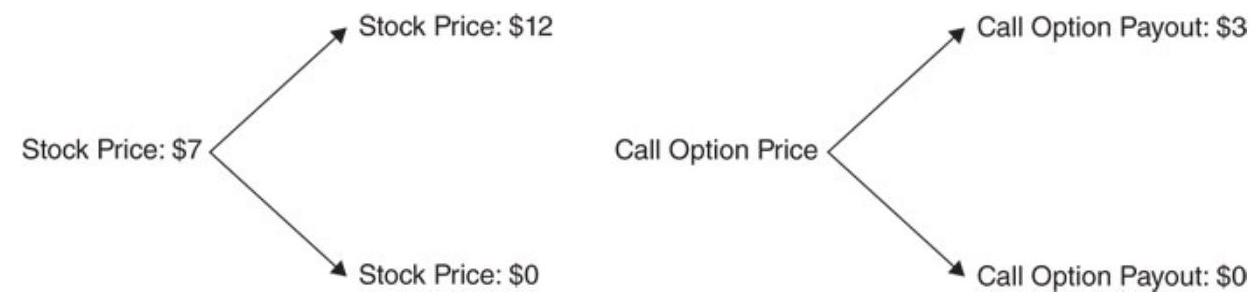
\includegraphics[max width=\textwidth, center]{2024_04_10_859893730bbb41b27826g-2(1)}

\section*{Binomial Trees for Stock and Call Option with $\$ 9$ Strike}
Without knowing the probability of the stock rising or falling, it is still possible to know the value of a one-year call option (or a put option), using the principles of arbitrage-free modeling. The solution is found by noting that in this specialized case, the payoff of the call option is always 0.25 times the payoff of the stock (i.e., $0.25 \times \$ 12=\$ 3$ ). Thus, the call option with a strike price of $\$ 9$ must sell for one-quarter the price of the stock, or $\$ 1.75$ (assuming no dividends). The idea is that four call options are economically equivalent to owning one share of stock, so that call option must sell for one-quarter the price of the stock.

\section*{The Nature and Power of a Risk-Neutral Model}
Note that the binomial model in the Binomial Trees for Stock and Call Option exhibit with a \$9 Strike was solved without specifying the probabilities of the up and down movements, without specifying the riskless interest rate, and without specifying the risk premium required for holding the stock. For example, perhaps the stock traded for $\$ 7$ because the interest rate was zero, the stock had no systematic risk (and therefore required no risk premium), and the stock had a $7 / 12$ ths chance of rising and a 5/12ths chance of becoming worthless. Perhaps the chance of the stock rising was 2/3rds but investors demanded a $14.29 \%$ expected return for holding the stock and therefore it traded at \$12. None of this matters, because the probabilities and interest rate were not required to find the solution.

A risk-neutral model is a framework for valuing financial derivatives in which risk preferences and probabilities of price changes do not alter the solution and are therefore irrelevant, and in which the analyst selects risk-neutrality as the model's underlying assumption with regard to risk preferences. Note that the probabilities and risk premiums can offset each other so there exist an infinite number of possible pairs of risk aversion and probabilities-two of which were given in the previous paragraph regarding the Binomial Trees for Stock and Call Option exhibit with a \$9 Strike. Given that there exists an infinite number of possible probabilities and risk premiums, an analyst can therefore pick the most convenient scenario-which is the risk-neutral scenario. In the risk-neutral scenario all discount rates are the riskless rate and all probabilities found are the ones that allow the price of the risky asset to match its model value.

Risk neutral models are a very important tool in valuing financial derivatives and are discussed in numerous places throughout this course and in Level II.

\section*{The Advantage to Binomial Tree Models and Their Extensions}
The primary advantage to binomial models is their flexibility to easily incorporate important features such as cash distributions, decisions by corporations to call (i.e., buy back) securities, and decisions by investors to exercise options prior to their expiration or to prepay loans.

In order to make the earlier binomial model extremely simple it was based on the highly unrealistic assumption that the stock price in one year would be either $\$ 12$ per share or zero. Obviously, actual binomial models relax that assumption. Binomial tree models can be based on interest rates (for valuing fixed-income securities), exchange rates (for currency derivatives), or two factors (e.g., interest rates and stock prices to value convertible bonds). Another extension is the use of trinomial models, in which each price is allowed to have three outcomes.


\end{document}